% Options for packages loaded elsewhere
% Options for packages loaded elsewhere
\PassOptionsToPackage{unicode}{hyperref}
\PassOptionsToPackage{hyphens}{url}
\PassOptionsToPackage{dvipsnames,svgnames,x11names}{xcolor}
%
\documentclass[
  letterpaper,
  DIV=11,
  numbers=noendperiod]{scrartcl}
\usepackage{xcolor}
\usepackage{amsmath,amssymb}
\setcounter{secnumdepth}{-\maxdimen} % remove section numbering
\usepackage{iftex}
\ifPDFTeX
  \usepackage[T1]{fontenc}
  \usepackage[utf8]{inputenc}
  \usepackage{textcomp} % provide euro and other symbols
\else % if luatex or xetex
  \usepackage{unicode-math} % this also loads fontspec
  \defaultfontfeatures{Scale=MatchLowercase}
  \defaultfontfeatures[\rmfamily]{Ligatures=TeX,Scale=1}
\fi
\usepackage{lmodern}
\ifPDFTeX\else
  % xetex/luatex font selection
\fi
% Use upquote if available, for straight quotes in verbatim environments
\IfFileExists{upquote.sty}{\usepackage{upquote}}{}
\IfFileExists{microtype.sty}{% use microtype if available
  \usepackage[]{microtype}
  \UseMicrotypeSet[protrusion]{basicmath} % disable protrusion for tt fonts
}{}
\makeatletter
\@ifundefined{KOMAClassName}{% if non-KOMA class
  \IfFileExists{parskip.sty}{%
    \usepackage{parskip}
  }{% else
    \setlength{\parindent}{0pt}
    \setlength{\parskip}{6pt plus 2pt minus 1pt}}
}{% if KOMA class
  \KOMAoptions{parskip=half}}
\makeatother
% Make \paragraph and \subparagraph free-standing
\makeatletter
\ifx\paragraph\undefined\else
  \let\oldparagraph\paragraph
  \renewcommand{\paragraph}{
    \@ifstar
      \xxxParagraphStar
      \xxxParagraphNoStar
  }
  \newcommand{\xxxParagraphStar}[1]{\oldparagraph*{#1}\mbox{}}
  \newcommand{\xxxParagraphNoStar}[1]{\oldparagraph{#1}\mbox{}}
\fi
\ifx\subparagraph\undefined\else
  \let\oldsubparagraph\subparagraph
  \renewcommand{\subparagraph}{
    \@ifstar
      \xxxSubParagraphStar
      \xxxSubParagraphNoStar
  }
  \newcommand{\xxxSubParagraphStar}[1]{\oldsubparagraph*{#1}\mbox{}}
  \newcommand{\xxxSubParagraphNoStar}[1]{\oldsubparagraph{#1}\mbox{}}
\fi
\makeatother


\usepackage{longtable,booktabs,array}
\newcounter{none} % for unnumbered tables
\usepackage{calc} % for calculating minipage widths
% Correct order of tables after \paragraph or \subparagraph
\usepackage{etoolbox}
\makeatletter
\patchcmd\longtable{\par}{\if@noskipsec\mbox{}\fi\par}{}{}
\makeatother
% Allow footnotes in longtable head/foot
\IfFileExists{footnotehyper.sty}{\usepackage{footnotehyper}}{\usepackage{footnote}}
\makesavenoteenv{longtable}
\usepackage{graphicx}
\makeatletter
\newsavebox\pandoc@box
\newcommand*\pandocbounded[1]{% scales image to fit in text height/width
  \sbox\pandoc@box{#1}%
  \Gscale@div\@tempa{\textheight}{\dimexpr\ht\pandoc@box+\dp\pandoc@box\relax}%
  \Gscale@div\@tempb{\linewidth}{\wd\pandoc@box}%
  \ifdim\@tempb\p@<\@tempa\p@\let\@tempa\@tempb\fi% select the smaller of both
  \ifdim\@tempa\p@<\p@\scalebox{\@tempa}{\usebox\pandoc@box}%
  \else\usebox{\pandoc@box}%
  \fi%
}
% Set default figure placement to htbp
\def\fps@figure{htbp}
\makeatother


% definitions for citeproc citations
\NewDocumentCommand\citeproctext{}{}
\NewDocumentCommand\citeproc{mm}{%
  \begingroup\def\citeproctext{#2}\cite{#1}\endgroup}
\makeatletter
 % allow citations to break across lines
 \let\@cite@ofmt\@firstofone
 % avoid brackets around text for \cite:
 \def\@biblabel#1{}
 \def\@cite#1#2{{#1\if@tempswa , #2\fi}}
\makeatother
\newlength{\cslhangindent}
\setlength{\cslhangindent}{1.5em}
\newlength{\csllabelwidth}
\setlength{\csllabelwidth}{3em}
\newenvironment{CSLReferences}[2] % #1 hanging-indent, #2 entry-spacing
 {\begin{list}{}{%
  \setlength{\itemindent}{0pt}
  \setlength{\leftmargin}{0pt}
  \setlength{\parsep}{0pt}
  % turn on hanging indent if param 1 is 1
  \ifodd #1
   \setlength{\leftmargin}{\cslhangindent}
   \setlength{\itemindent}{-1\cslhangindent}
  \fi
  % set entry spacing
  \setlength{\itemsep}{#2\baselineskip}}}
 {\end{list}}
\usepackage{calc}
\newcommand{\CSLBlock}[1]{\hfill\break\parbox[t]{\linewidth}{\strut\ignorespaces#1\strut}}
\newcommand{\CSLLeftMargin}[1]{\parbox[t]{\csllabelwidth}{\strut#1\strut}}
\newcommand{\CSLRightInline}[1]{\parbox[t]{\linewidth - \csllabelwidth}{\strut#1\strut}}
\newcommand{\CSLIndent}[1]{\hspace{\cslhangindent}#1}



\setlength{\emergencystretch}{3em} % prevent overfull lines

\providecommand{\tightlist}{%
  \setlength{\itemsep}{0pt}\setlength{\parskip}{0pt}}



 


\usepackage{float}
\usepackage{tabularray}
\usepackage[normalem]{ulem}
\usepackage{graphicx}
\usepackage{rotating}
\UseTblrLibrary{siunitx}
\NewTableCommand{\tinytableDefineColor}[3]{\definecolor{#1}{#2}{#3}}
\newcommand{\tinytableTabularrayUnderline}[1]{\underline{#1}}
\newcommand{\tinytableTabularrayStrikeout}[1]{\sout{#1}}
\usepackage{float}
\floatplacement{table}{H}
\KOMAoption{captions}{tableheading}
\makeatletter
\@ifpackageloaded{caption}{}{\usepackage{caption}}
\AtBeginDocument{%
\ifdefined\contentsname
  \renewcommand*\contentsname{Table of contents}
\else
  \newcommand\contentsname{Table of contents}
\fi
\ifdefined\listfigurename
  \renewcommand*\listfigurename{List of Figures}
\else
  \newcommand\listfigurename{List of Figures}
\fi
\ifdefined\listtablename
  \renewcommand*\listtablename{List of Tables}
\else
  \newcommand\listtablename{List of Tables}
\fi
\ifdefined\figurename
  \renewcommand*\figurename{Figure}
\else
  \newcommand\figurename{Figure}
\fi
\ifdefined\tablename
  \renewcommand*\tablename{Table}
\else
  \newcommand\tablename{Table}
\fi
}
\@ifpackageloaded{float}{}{\usepackage{float}}
\floatstyle{ruled}
\@ifundefined{c@chapter}{\newfloat{codelisting}{h}{lop}}{\newfloat{codelisting}{h}{lop}[chapter]}
\floatname{codelisting}{Listing}
\newcommand*\listoflistings{\listof{codelisting}{List of Listings}}
\makeatother
\makeatletter
\makeatother
\makeatletter
\@ifpackageloaded{caption}{}{\usepackage{caption}}
\@ifpackageloaded{subcaption}{}{\usepackage{subcaption}}
\makeatother
\usepackage{bookmark}
\IfFileExists{xurl.sty}{\usepackage{xurl}}{} % add URL line breaks if available
\urlstyle{same}
% fallback for those not using the hyperref driver hyperxmp:
\makeatletter
\@ifundefined{xmpquote}{\newcommand{\xmpquote}[1]{#1}}{}
\makeatother
\hypersetup{
  pdftitle={Communicable Diseases in Toronto: Trends and Implications for Prevention},
  pdfauthor={Joshua Campbell},
  colorlinks=true,
  linkcolor={blue},
  filecolor={Maroon},
  citecolor={Blue},
  urlcolor={Blue},
  pdfcreator={LaTeX via pandoc}}


\title{Communicable Diseases in Toronto: Trends and Implications for
Prevention\footnote{All code and data are available at:
  https://github.com/JoshECampbell/Toronto-Communicable-Disease-Report.}}
\author{Joshua Campbell}
\date{28 September 2026}
\begin{document}
\maketitle


Communicable disease surveillance programs can help public health
agencies track changes in reported illness and plan prevention efforts
around recurring seasonal patterns. This report examines Toronto's
Monthly Communicable Disease Surveillance Data from 2021 to 2025,
comparing monthly case totals across six disease categories and annual
influenza rates. The categories show different seasonal patterns;
influenza closely follows the winter peaks in vaccine-preventable
disease cases and reached an annual rate of 387.0 cases per 100,000 in
2025. These findings show how surveillance data can support monitoring
across diseases and help time influenza vaccination outreach before the
winter increase.

\section{1. Introduction}\label{introduction}

Communicable disease surveillance plays an important role in
understanding how infectious diseases affect a population over time. By
tracking reported cases over time, public health agencies can identify
emerging patterns and support decision-making related to public health
programming (City of Toronto 2025). In Toronto, Toronto Public Health
(TPH) publishes a monthly surveillance dataset describing reported cases
of a wide range of communicable diseases (Toronto Public Health 2026).

This report analyzes TPH's Monthly Communicable Disease Surveillance
Data for the years 2021 through 2025, excluding data associated with
COVID-19. It compares monthly reported cases across six disease
categories, examines influenza's contribution to vaccine-preventable
disease peaks, and considers annual influenza rates alongside national
vaccination coverage estimates.

Because the timing and volume of reported cases differ by disease,
annual totals alone cannot show when outreach may be most useful or
which disease accounts for a category's increase. Comparing monthly
patterns across categories shows that vaccine-preventable cases peak in
winter, and that reported cases of influenza account for most of the
volume within the category. A closer look at influenza shows that its
population-adjusted annual rate also rose sharply from 2024 to 2025.

These findings show how monthly surveillance can help track seasonal
patterns and flag unusual increases across diseases. The influenza
pattern can also help TPH plan vaccination outreach before winter
activity rises. Section 2 presents the data and observed trends while
Section 3 discusses their implications for disease monitoring and
vaccination outreach.

\section{2. Data}\label{data}

\subsection{2.1 Toronto Communicable Disease Surveillance
Data}\label{toronto-communicable-disease-surveillance-data}

Toronto Public Health (TPH) is responsible for updating and publishing a
monthly dataset that describes reported cases of communicable diseases
within the City of Toronto. These datasets are made available through
the City of Toronto's Open Data Portal under the title ``Monthly
Communicable Disease Surveillance Data'' (Toronto Public Health 2026).

As outlined by TPH, health surveillance programs, such as this one, help
identify current public health issues. They also provide evidence to
inform policy decisions aimed at reducing health risks and improving
population health outcomes (City of Toronto 2025). Similarly to TPH,
Public Health Ontario (PHO) also provides information on reported
disease cases for a variety of infectious diseases, filtered by region
(Public Health Ontario 2026). The PHO dataset serves as an alternative
to the one used for this report and can be used to expand the analysis
to investigate similar trends across multiple health units across
Ontario.

Reports from 2021 to 2026 were downloaded using the statistical
programming language \texttt{R} (R Core Team 2026), with select packages
\texttt{dplyr}, \texttt{here} and \texttt{glue} (Wickham et al. 2026)
(Hester and Bryan 2026) (Müller 2025). The analysis includes complete
calendar years from 2021 to 2025, with revised 2025 annual counts and
rates taken from the 2026 report.

\texttt{Python} was used to combine the reports into one dataset with a
row for each disease and year (Python Software Foundation 2026). The
rows correspond to reported case counts for a selected disease and year.
Rows corresponding to COVID-19 were not included as they were out of the
scope of this report. The cleaned dataset consists of 331 rows,
including 79 unique diseases across 6 distinct categories. An outline of
the variables as well as their descriptions can be found in
Table~\ref{tbl-variables} and a sample of the dataset can be found in
Table~\ref{tbl-sample}.

\begin{table}

\caption{\label{tbl-variables}Fields found in the cleaned dataset with
corresponding descriptions.}

\centering{

\centering
\begin{tblr}[         %% tabularray outer open
]                     %% tabularray outer close
{                     %% tabularray inner open
colspec={Q[]Q[]},
hline{2}={1-2}{solid, black, 0.05em},
hline{1}={1-2}{solid, black, 0.08em},
hline{8}={1-2}{solid, black, 0.08em},
}                     %% tabularray inner close
Variable & Description \\
Disease & Name of reported disease. \\
Disease Category & The reporting category assigned to the disease. \\
January-December & Reported case counts for the months of the calendar year. \\
Yearly Cases & Reported case counts for the year of surveillance for a given disease. \\
Yearly Rate & Yearly rate expressed as yearly cases per 100,000 population. \\
Year & Year of observation. \\
\end{tblr}

}

\end{table}%

\subsection{2.2 Monthly Disease-Category
Patterns}\label{monthly-disease-category-patterns}

The monthly series of cases at the disease-category level provides a
detailed view of how reported communicable diseases evolve between
January 2021 and December 2025. For each category, monthly case totals
are constructed by summing the reported cases of diseases assigned to
that group. The resulting series therefore represents reported cases
rather than unique individuals, since an individual may appear more than
once across diseases. The diseases found within each disease category
are summarized in Table~\ref{tbl-disease-categories}.

\begin{table}

\caption{\label{tbl-disease-categories}Diseases included in each
category, 2021--2025.}

\centering{

\centering
\begin{talltblr}[         %% tabularray outer open
entry=none,label=none,
note{}={* Not listed in every year from 2021 to 2025.},
]                     %% tabularray outer close
{                     %% tabularray inner open
width={1\linewidth},
colspec={X[0.25]X[0.75]},
hline{2}={1-2}{solid, black, 0.05em},
hline{1}={1-2}{solid, black, 0.08em},
hline{8}={1-2}{solid, black, 0.08em},
}                     %% tabularray inner close
Disease Category & Diseases \\
Diseases Transmitted by Direct Contact and Respiratory Routes & Group A Streptococcal disease, invasive (iGAS); Group B Streptococcal disease, neonatal (GBS); Legionellosis; Leprosy; Mpox*; SARS*; TB: Atypical mycobacterial infections*; Tuberculosis; Tuberculosis infection, latent (LTBI)* \\
Enteric Food and Waterborne Diseases & Amebiasis; Botulism; Campylobacter enteritis; Cholera; Cryptosporidiosis; Cyclosporiasis; Food poisoning; Giardiasis; Hepatitis A; Listeriosis; Paralytic shellfish poisoning; Paratyphoid fever; Salmonellosis; Shigellosis; Trichinosis; Typhoid fever; Verotoxin-producing E. coli infection (VTEC); Yersiniosis \\
Other Diseases & Blastomycosis; Candida auris*; Carbapenemase-producing Enterobacteriaceae (CPE); Creutzfeldt-Jakob disease (CJD) \\
Sexually Transmitted and Bloodborne Infections & AIDS; Chancroid; Chlamydia; Gonorrhea; HIV; Hepatitis B carriers; Hepatitis B cases; Hepatitis B unclassified reports; Hepatitis C; Ophthalmia neonatorum; Syphilis, early congenital*; Syphilis, infectious; Syphilis, late congenital*; Syphilis, late latent*; Syphilis, other; Syphilitic stillbirth* \\
Vaccine Preventable Diseases & Acute flaccid paralysis; Adverse vaccine reactions*; Chickenpox (Varicella); Diphtheria; Haemophilus influenzae, invasive (all types); Influenza; Measles; Meningococcal disease, invasive (IMD); Mumps; Pertussis (Whooping Cough); Pneumococcal disease, invasive (IPD); Poliomyelitis*; Rubella; Rubella, congenital syndrome (CRS); Smallpox*; Tetanus \\
Vectorborne and Zoonotic Diseases & Anaplasmosis*; Anthrax*; Babesiosis*; Brucellosis; Echinococcus multilocularis infection; Hantavirus*; Hemorrhagic fevers; Lassa fever*; Lyme disease; Plague*; Powassan virus*; Psittacosis/Ornithosis*; Q fever; Rabies; Tularemia; West Nile Virus (WNV) \\
\end{talltblr}

}

\end{table}%

\begin{figure}[H]

\centering{

\pandocbounded{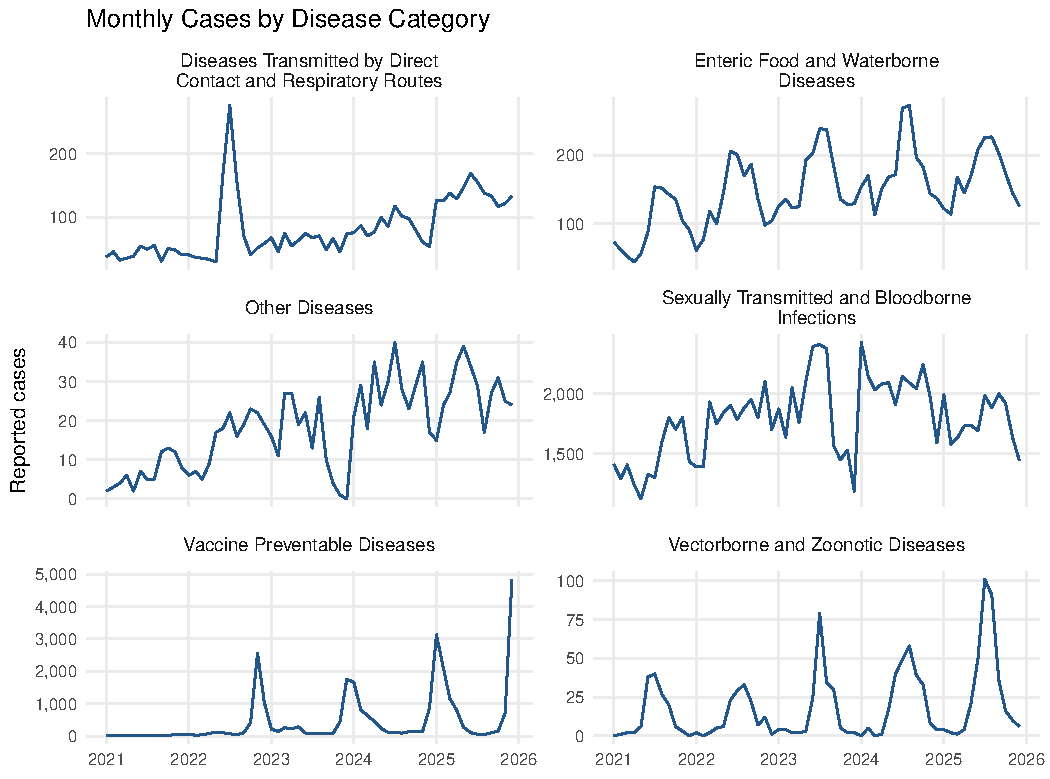
\includegraphics[keepaspectratio]{paper_files/figure-pdf/fig-monthly-disease-categories-1.pdf}}

}

\caption{\label{fig-monthly-disease-categories}Monthly reported cases by
category, 2021-2025. Panels use different vertical scales.}

\end{figure}%

The monthly series shows substantial differences in both the volume and
timing of reported cases across categories
(Figure~\ref{fig-monthly-disease-categories}). Certain categories show a
stronger seasonal structure. Most notably, vaccine-preventable cases are
concentrated near the end and beginning of the calendar year, with
distinct annual peaks occurring in December and January (December 2023,
January 2024, December 2025). In contrast, enteric, food and waterborne
diseases and vector-borne and zoonotic diseases rise during the summer
months, with the latter peaking in July or August. The contrast shows
why annual totals alone are insufficient to describe the timing of
reported illness. Comparing new months with earlier seasonal patterns
can flag unusual increases for closer investigation.

Comparing category totals with disease-level counts helps show which
diseases account for seasonal peaks. Influenza provides an example
within the vaccine-preventable category.

\subsection{2.3 Influenza and Vaccine-Preventable
Diseases}\label{influenza-and-vaccine-preventable-diseases}

Between 2022 and 2025, influenza accounted for 81.4\% to 94.1\% of
reported vaccine-preventable disease cases.
Figure~\ref{fig-influenza-vaccine-dep} illustrates this relationship as
the monthly curve for influenza closely follows the overall category's
peaks. The low influenza count in 2021 is an exception, so the pattern
cannot be described as uniform across all five years. Comparing the two
curves shows how much of the category's seasonal variation is associated
with this single disease.

\begin{figure}[H]

\centering{

\pandocbounded{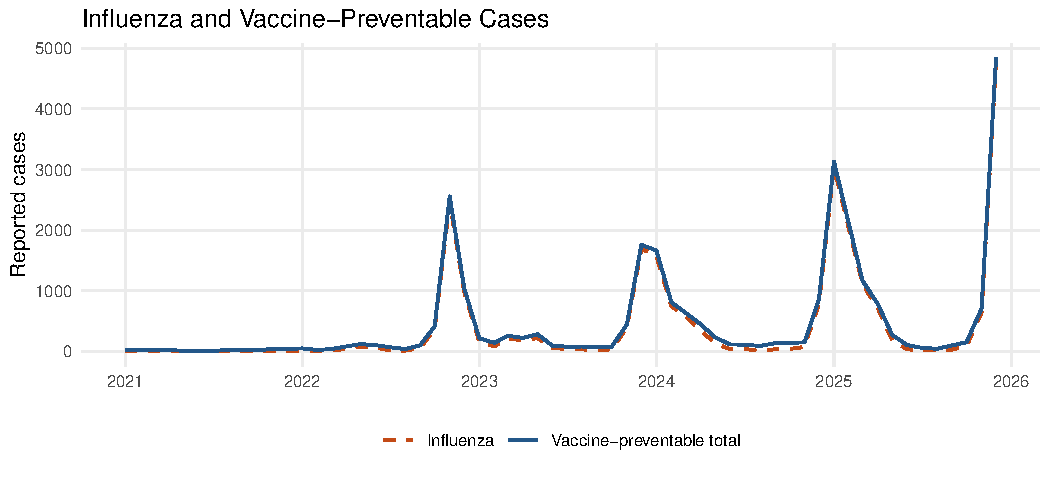
\includegraphics[keepaspectratio]{paper_files/figure-pdf/fig-influenza-vaccine-dep-1.pdf}}

}

\caption{\label{fig-influenza-vaccine-dep}Monthly influenza cases and
the vaccine-preventable category total, 2021-2025.}

\end{figure}%

The annual influenza rate declined to 105.8 per 100,000 in 2023, then
increased to 148.3 in 2024 and 387.0 in 2025, the highest value
observed. The increase from 2024 to 2025 is especially noticeable,
showing that much of the recent rise occurred in the final year rather
than building gradually across the whole period. This jump in
population-adjusted rates suggests the increased case counts during
seasonal peaks cannot be completely explained by population growth.

\begin{figure}[H]

\centering{

\pandocbounded{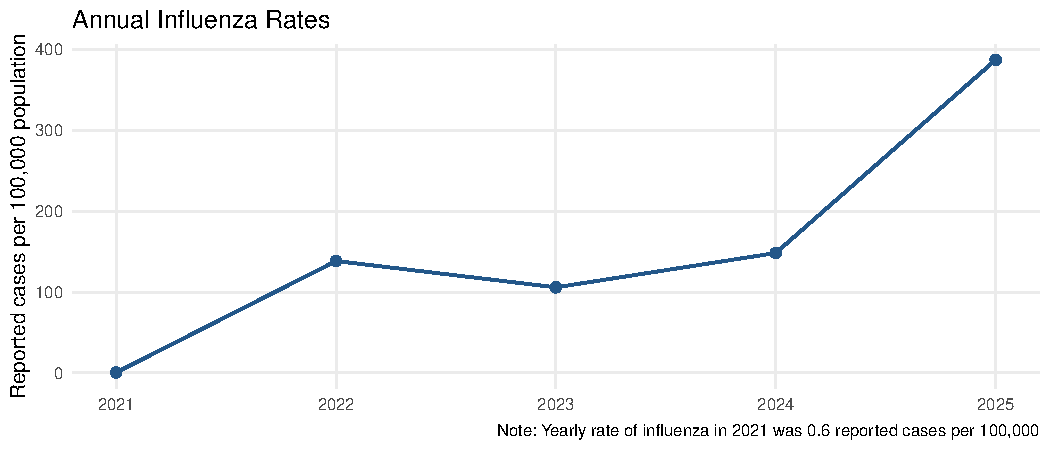
\includegraphics[keepaspectratio]{paper_files/figure-pdf/fig-influenza-yearly-rate-1.pdf}}

}

\caption{\label{fig-influenza-yearly-rate}Annual reported influenza
rates, 2021-2025.}

\end{figure}%

\section{3. Discussion}\label{discussion}

\subsection{3.1 Reported Influenza Cases and Vaccination
Coverage}\label{reported-influenza-cases-and-vaccination-coverage}

The category comparisons show how monthly surveillance can be used
across diseases. Summer increases in enteric, food and waterborne
diseases and vector-borne and zoonotic diseases can be monitored against
their usual seasonal timing. An unusual increase in any category can
prompt closer review of individual diseases and case reports, though
these patterns alone cannot establish whether an outbreak has occurred.
For vaccine-preventable diseases, the recurring winter increase also
provides a practical window for prevention efforts.

Influenza accounted for most reported vaccine-preventable disease cases
between 2022 and 2025, and its annual rate increased sharply in 2025.
The increase in population-adjusted rates indicates that population
growth alone does not explain the rise in reported cases. Influenza
vaccination is therefore a relevant focus for outreach before winter
activity increases, although vaccination coverage is not measured in the
Toronto dataset (Toronto Public Health 2026).

According to the Public Health Agency of Canada (PHAC), annual influenza
vaccination is recommended for nearly everyone aged six months and older
and reduces the risk of infection and flu-related complications.
Vaccination also helps limit transmission to others, including those who
are at greater risk of severe illness. PHAC identifies people aged 65
and older and adults aged 18-64 with chronic medical conditions as
higher risk (Public Health Agency of Canada 2025). The national
influenza vaccination coverage target is 80\% for the two populations
(Public Health Agency of Canada 2026b).

PHAC reports that vaccination among adults aged 18-64 without chronic
medical conditions was under one third of the population from 2021
through 2025. In 2024-2025, coverage was 32.3\% among adults aged 18-64
with chronic conditions and 63.2\% among adults aged 65 and older
(Public Health Agency of Canada 2026b).

For the 2025-2026 season, the survey found the main reasons for
non-vaccination were the perception of good health, followed by ``not
getting round to it'' (Public Health Agency of Canada 2026b). This may
point to a gap in community outreach, particularly in communicating the
importance of annual influenza vaccination to people who are not
considered high-risk. In 2025, the Ministry of Health issued an
executive notice announcing that publicly funded influenza vaccines were
available in pharmacies across Ontario (Ontario Ministry of Health
2025). However, improving access alone may not be sufficient to increase
vaccine uptake. Additional resources could therefore be directed toward
reducing barriers to participation, including targeted communication
campaigns and convenient vaccination clinics available in workplaces and
on campuses.

Timing also matters. Influenza's largest spikes occurred in December
2023, January 2024 and December 2025. Protective antibody levels
generally develop about two weeks after vaccination, and influenza
vaccination is recommended annually (Public Health Agency of Canada
2026a). These observed peaks support planning outreach early in autumn
and encouraging vaccination when eligible and available, allowing time
for an immune response before seasonal activity increases. Continued
monthly monitoring can show whether the timing or scale of future
increases differs from earlier years.

\subsection{3.2 Limitations}\label{limitations}

A limitation of this analysis is its dependence on consistent reporting
and testing for the diseases recorded. Additionally, national coverage
estimates may not generalize to the population of Toronto and cannot
show that low vaccination uptake caused the city's increase in
influenza.

\section{Appendix}\label{appendix}

\subsection{A. Sample Data}\label{a.-sample-data}

\begin{table}

\caption{\label{tbl-sample}Sample entries from the cleaned dataset.}

\centering{

\centering
\begin{talltblr}[         %% tabularray outer open
entry=none,label=none,
note{}={Note: January and December illustrate the monthly fields. Rates are per 100,000 population.},
]                     %% tabularray outer close
{                     %% tabularray inner open
width={0.9\linewidth},
colspec={X[0.18]X[0.24]X[0.08]X[0.08]X[0.08]X[0.12]X[0.12]},
hline{2}={1-7}{solid, black, 0.05em},
hline{1}={1-7}{solid, black, 0.08em},
hline{6}={1-7}{solid, black, 0.08em},
column{1-7}={}{font=\fontsize{0.7em}{1em}\selectfont},
}                     %% tabularray inner close
Category & Disease & Year & Jan & Dec & Cases & Rate \\
Diseases Transmitted by Direct Contact and Respiratory Routes & Group A Streptococcal disease, invasive (iGAS) & 2021 & 14 & 13 & 119 & 4.0 \\
Diseases Transmitted by Direct Contact and Respiratory Routes & Group B Streptococcal disease, neonatal (GBS) & 2025 & 0 & 0 & 5 & 19.1 \\
Enteric Food and Waterborne Diseases & Salmonellosis & 2025 & 36 & 30 & 494 & 15.1 \\
Vaccine Preventable Diseases & Rubella & 2025 & 0 & 0 & 0 & 0.0 \\
\end{talltblr}

}

\end{table}%

\section*{References}\label{references}
\addcontentsline{toc}{section}{References}

\protect\phantomsection\label{refs}
\begin{CSLReferences}{1}{1}
\bibitem[\citeproctext]{ref-HSP_2026}
City of Toronto. 2025. {``Health Surveillance and Epidemiology
Reports.''} In \emph{City of Toronto}.
\url{https://www.toronto.ca/city-government/data-research-maps/research-reports/public-health-significant-reports/health-surveillance-and-epidemiology-reports/}.

\bibitem[\citeproctext]{ref-glue2026}
Hester, Jim, and Jennifer Bryan. 2026. \emph{Glue: Interpreted String
Literals}. \url{https://doi.org/10.32614/CRAN.package.glue}.

\bibitem[\citeproctext]{ref-here2025}
Müller, Kirill. 2025. \emph{Here: A Simpler Way to Find Your Files}.
\url{https://doi.org/10.32614/CRAN.package.here}.

\bibitem[\citeproctext]{ref-ontarioInfluenza2025}
Ontario Ministry of Health. 2025. \emph{Executive Officer Notice:
Administration of Publicly Funded Influenza Vaccines in Ontario
Pharmacies}.
\url{https://www.ontario.ca/files/2025-10/moh-executive-officer-notice-en-2025-10-15.pdf}.

\bibitem[\citeproctext]{ref-phacFluShot}
Public Health Agency of Canada. 2025. \emph{Get Your Flu Shot}.
\url{https://www.canada.ca/en/public-health/services/diseases/flu-influenza/get-your-flu-shot.html}.

\bibitem[\citeproctext]{ref-phacInfluenzaGuide}
Public Health Agency of Canada. 2026a. \emph{Influenza Vaccines:
Canadian Immunization Guide}.
\url{https://www.canada.ca/en/public-health/services/publications/healthy-living/canadian-immunization-guide-part-4-active-vaccines/page-10-influenza-vaccine.html}.

\bibitem[\citeproctext]{ref-canada_srvcs_2026}
Public Health Agency of Canada. 2026b. {``Seasonal Respiratory
Vaccination Coverage Survey (SRVCS): Vaccination Coverage Report.''}
\url{https://health-infobase.canada.ca/vaccination/seasonal-respiratory-vaccination-coverage-survey/report.html}.

\bibitem[\citeproctext]{ref-phoDiseaseTrends2026}
Public Health Ontario. 2026. \emph{Infectious Disease Trends in Ontario
Tool}.
\url{https://www.publichealthontario.ca/en/Data-and-Analysis/Infectious-Disease/Reportable-Disease-Trends-Annually}.

\bibitem[\citeproctext]{ref-python2026}
Python Software Foundation. 2026. \emph{{Python} Programming Language}.
\url{https://www.python.org/downloads/release/python-3147/}.

\bibitem[\citeproctext]{ref-r2026}
R Core Team. 2026. \emph{R: A Language and Environment for Statistical
Computing}. R Foundation for Statistical Computing.
\url{https://doi.org/10.32614/R.manuals}.

\bibitem[\citeproctext]{ref-torontoCommunicableData}
Toronto Public Health. 2026. \emph{Monthly Communicable Disease
Surveillance Data}. City of Toronto Open Data.
\url{https://open.toronto.ca/dataset/monthly-communicable-disease-surveillance-data/}.

\bibitem[\citeproctext]{ref-dplyr2026}
Wickham, Hadley, Romain François, Lionel Henry, Kirill Müller, and Davis
Vaughan. 2026. \emph{Dplyr: A Grammar of Data Manipulation}.
\url{https://doi.org/10.32614/CRAN.package.dplyr}.

\end{CSLReferences}




\end{document}
